
%使用XeLaTeX编译
%版权所有,翻版必究
%本文件由程序自动生成,任何修改将被覆盖
%2019 年 01 月 23 日




\FloatBarrier
\section{
导引
}\label{c000015s000001}


%begin图片
\begin{figure}[htb] %浮动体 here and top ...
%there must use marginnote ...
\marginnote{\setlength\fboxsep{2pt}\fbox{\footnotesize{\kaishu\figurename\,}\footnotesize{\ref{p000012}}}}\centering %中心对齐
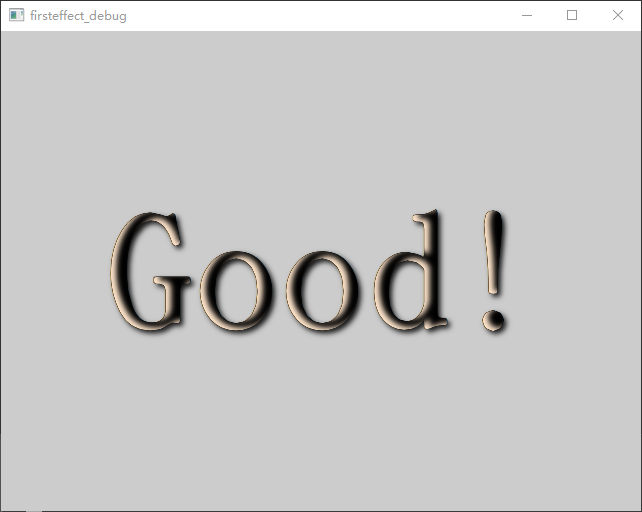
\includegraphics[width=0.95\textwidth]{../chapter06/firsteffect/the_app.png} %图片路径
\caption{文字阴影} %标题
\label{p000012} %索引
\end{figure}
%end图片


aaaaaaaaaaaaaaaaaaaaaaaa

%使用XeLaTeX编译
%版权所有,翻版必究
%本文件由程序自动生成,任何修改将被覆盖
%2019 年 01 月 23 日



%表
\begin{longtable}{ccc}

%表头....
\toprule{}类名 
&
分类
&
简介%there must use marginnote ...
\marginnote{\setlength\fboxsep{2pt}\fbox{\footnotesize{\kaishu\tablename\,}\footnotesize{\ref{tb000000}}}}
\\ \midrule 
\endfirsthead

%表尾...
\bottomrule
\caption{ThresholdMask}\label{tb000000} 
\endlastfoot

%重复表头
\toprule{}类名 
&
分类
&
简介
\\ \midrule
\endhead
%重复表尾
\midrule
\endfoot 
Blend & aabbc & cccc \\
BrightnessContrast & aabbc & cccc \\
ColorOverlay & aabbc & cccc \\
Colorize & aabbc & cccc \\
Desaturate & aabbc & cccc \\
GammaAdjust & aabbc & cccc \\
HueSaturation & aabbc & cccc \\
LevelAdjust & aabbc & cccc \\
ConicalGradient & aabbc & cccc \\
LinearGradient & aabbc & cccc \\
RadialGradient & aabbc & cccc \\
Displace & aabbc & cccc \\
DropShadow & aabbc & cccc \\
InnerShadow & aabbc & cccc \\
FastBlur & aabbc & cccc \\
GaussianBlur & aabbc & cccc \\
MaskedBlur & aabbc & cccc \\
RecursiveBlur & aabbc & cccc \\
DirectionalBlur & aabbc & cccc \\
RadialBlur & aabbc & cccc \\
ZoomBlur & aabbc & cccc \\
Glow & aabbc & cccc \\
RectangularGlow & aabbc & cccc \\
OpacityMask & aabbc & cccc \\
ThresholdMask  & aabbc & cccc \\
\end{longtable}
%表





%使用XeLaTeX编译
%版权所有,翻版必究
%本文件由程序自动生成,任何修改将被覆盖
%2019 年 01 月 23 日




bbbbbbbbbbbbbbbbbbbbbbbb






%使用XeLaTeX编译
%版权所有,翻版必究
%本文件由程序自动生成,任何修改将被覆盖
%2019 年 01 月 23 日



